\appendix{Представление графического материала}

Графический материал, выполненный на отдельных листах,
изображен на рисунках А.1--А.\arabic{числоПлакатов}.
\setcounter{числоПлакатов}{0}

\renewcommand{\thefigure}{А.\arabic{figure}} % шаблон номера для плакатов

\begin{landscape}

\begin{плакат}
    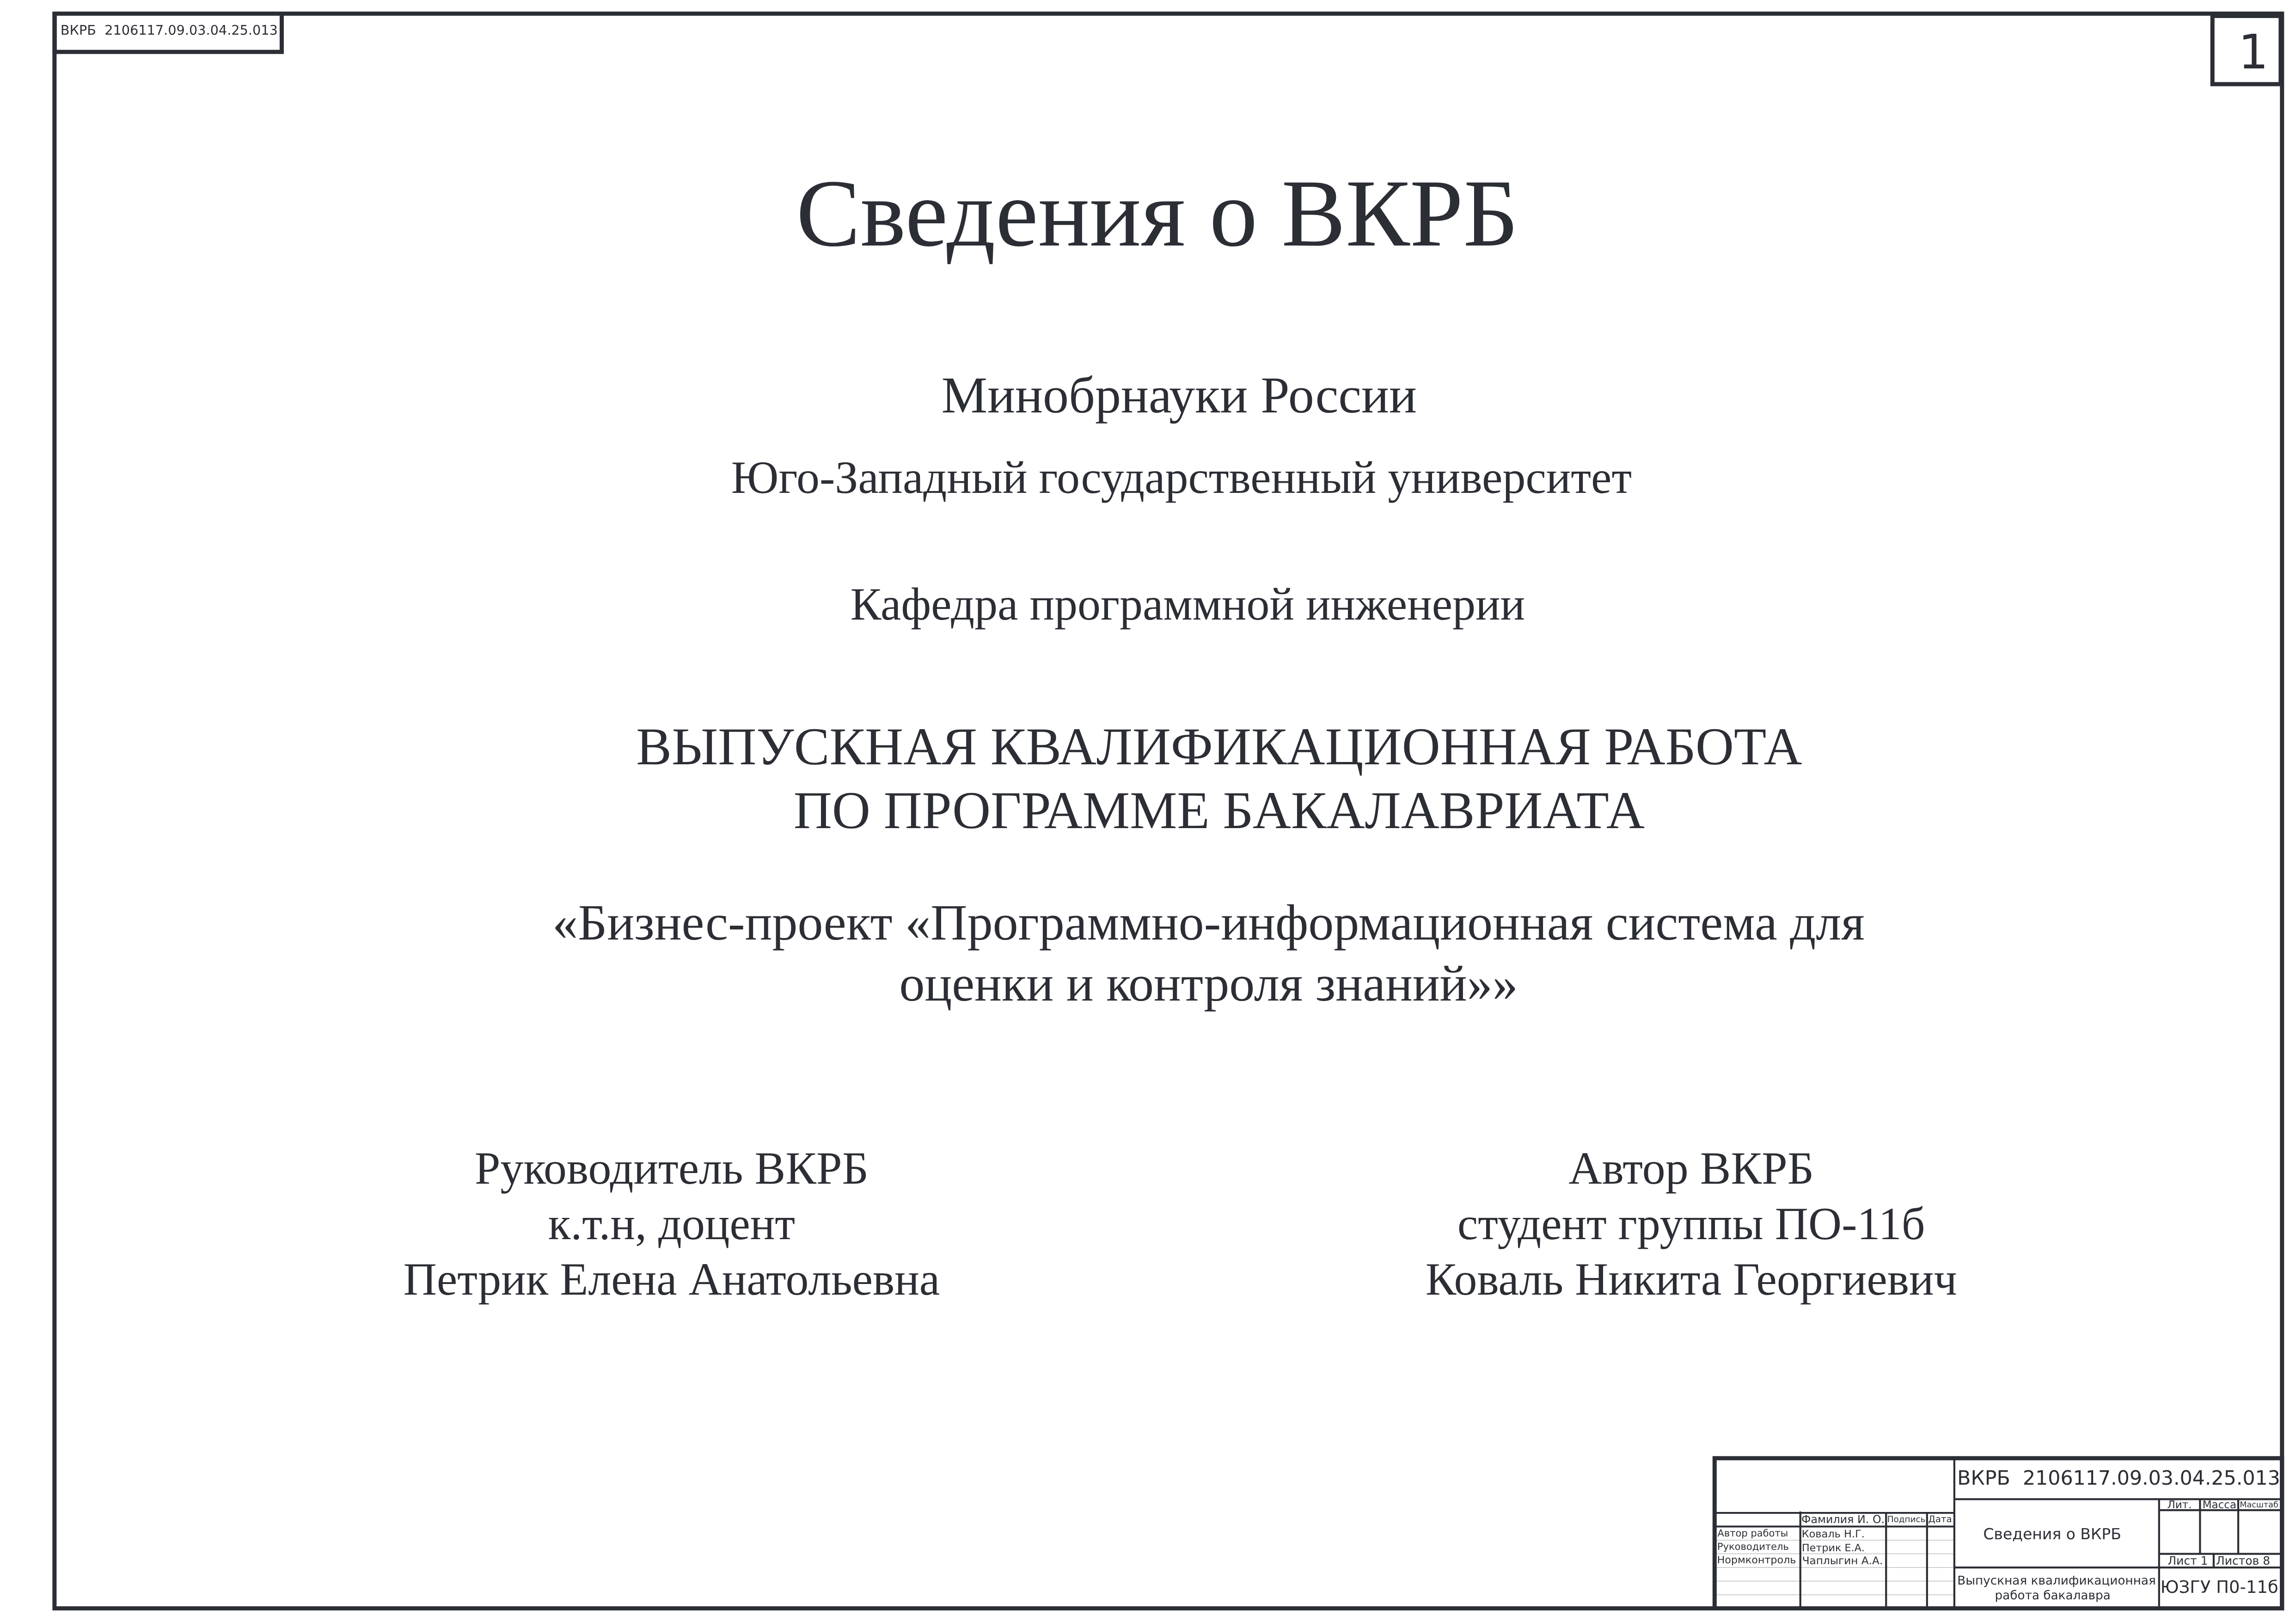
\includegraphics[width=0.82\linewidth]{Плакат_ВКР.eps}
    \заголовок{Сведения о ВКРБ}
    \label{pl1:image}      
\end{плакат}

\begin{плакат}
    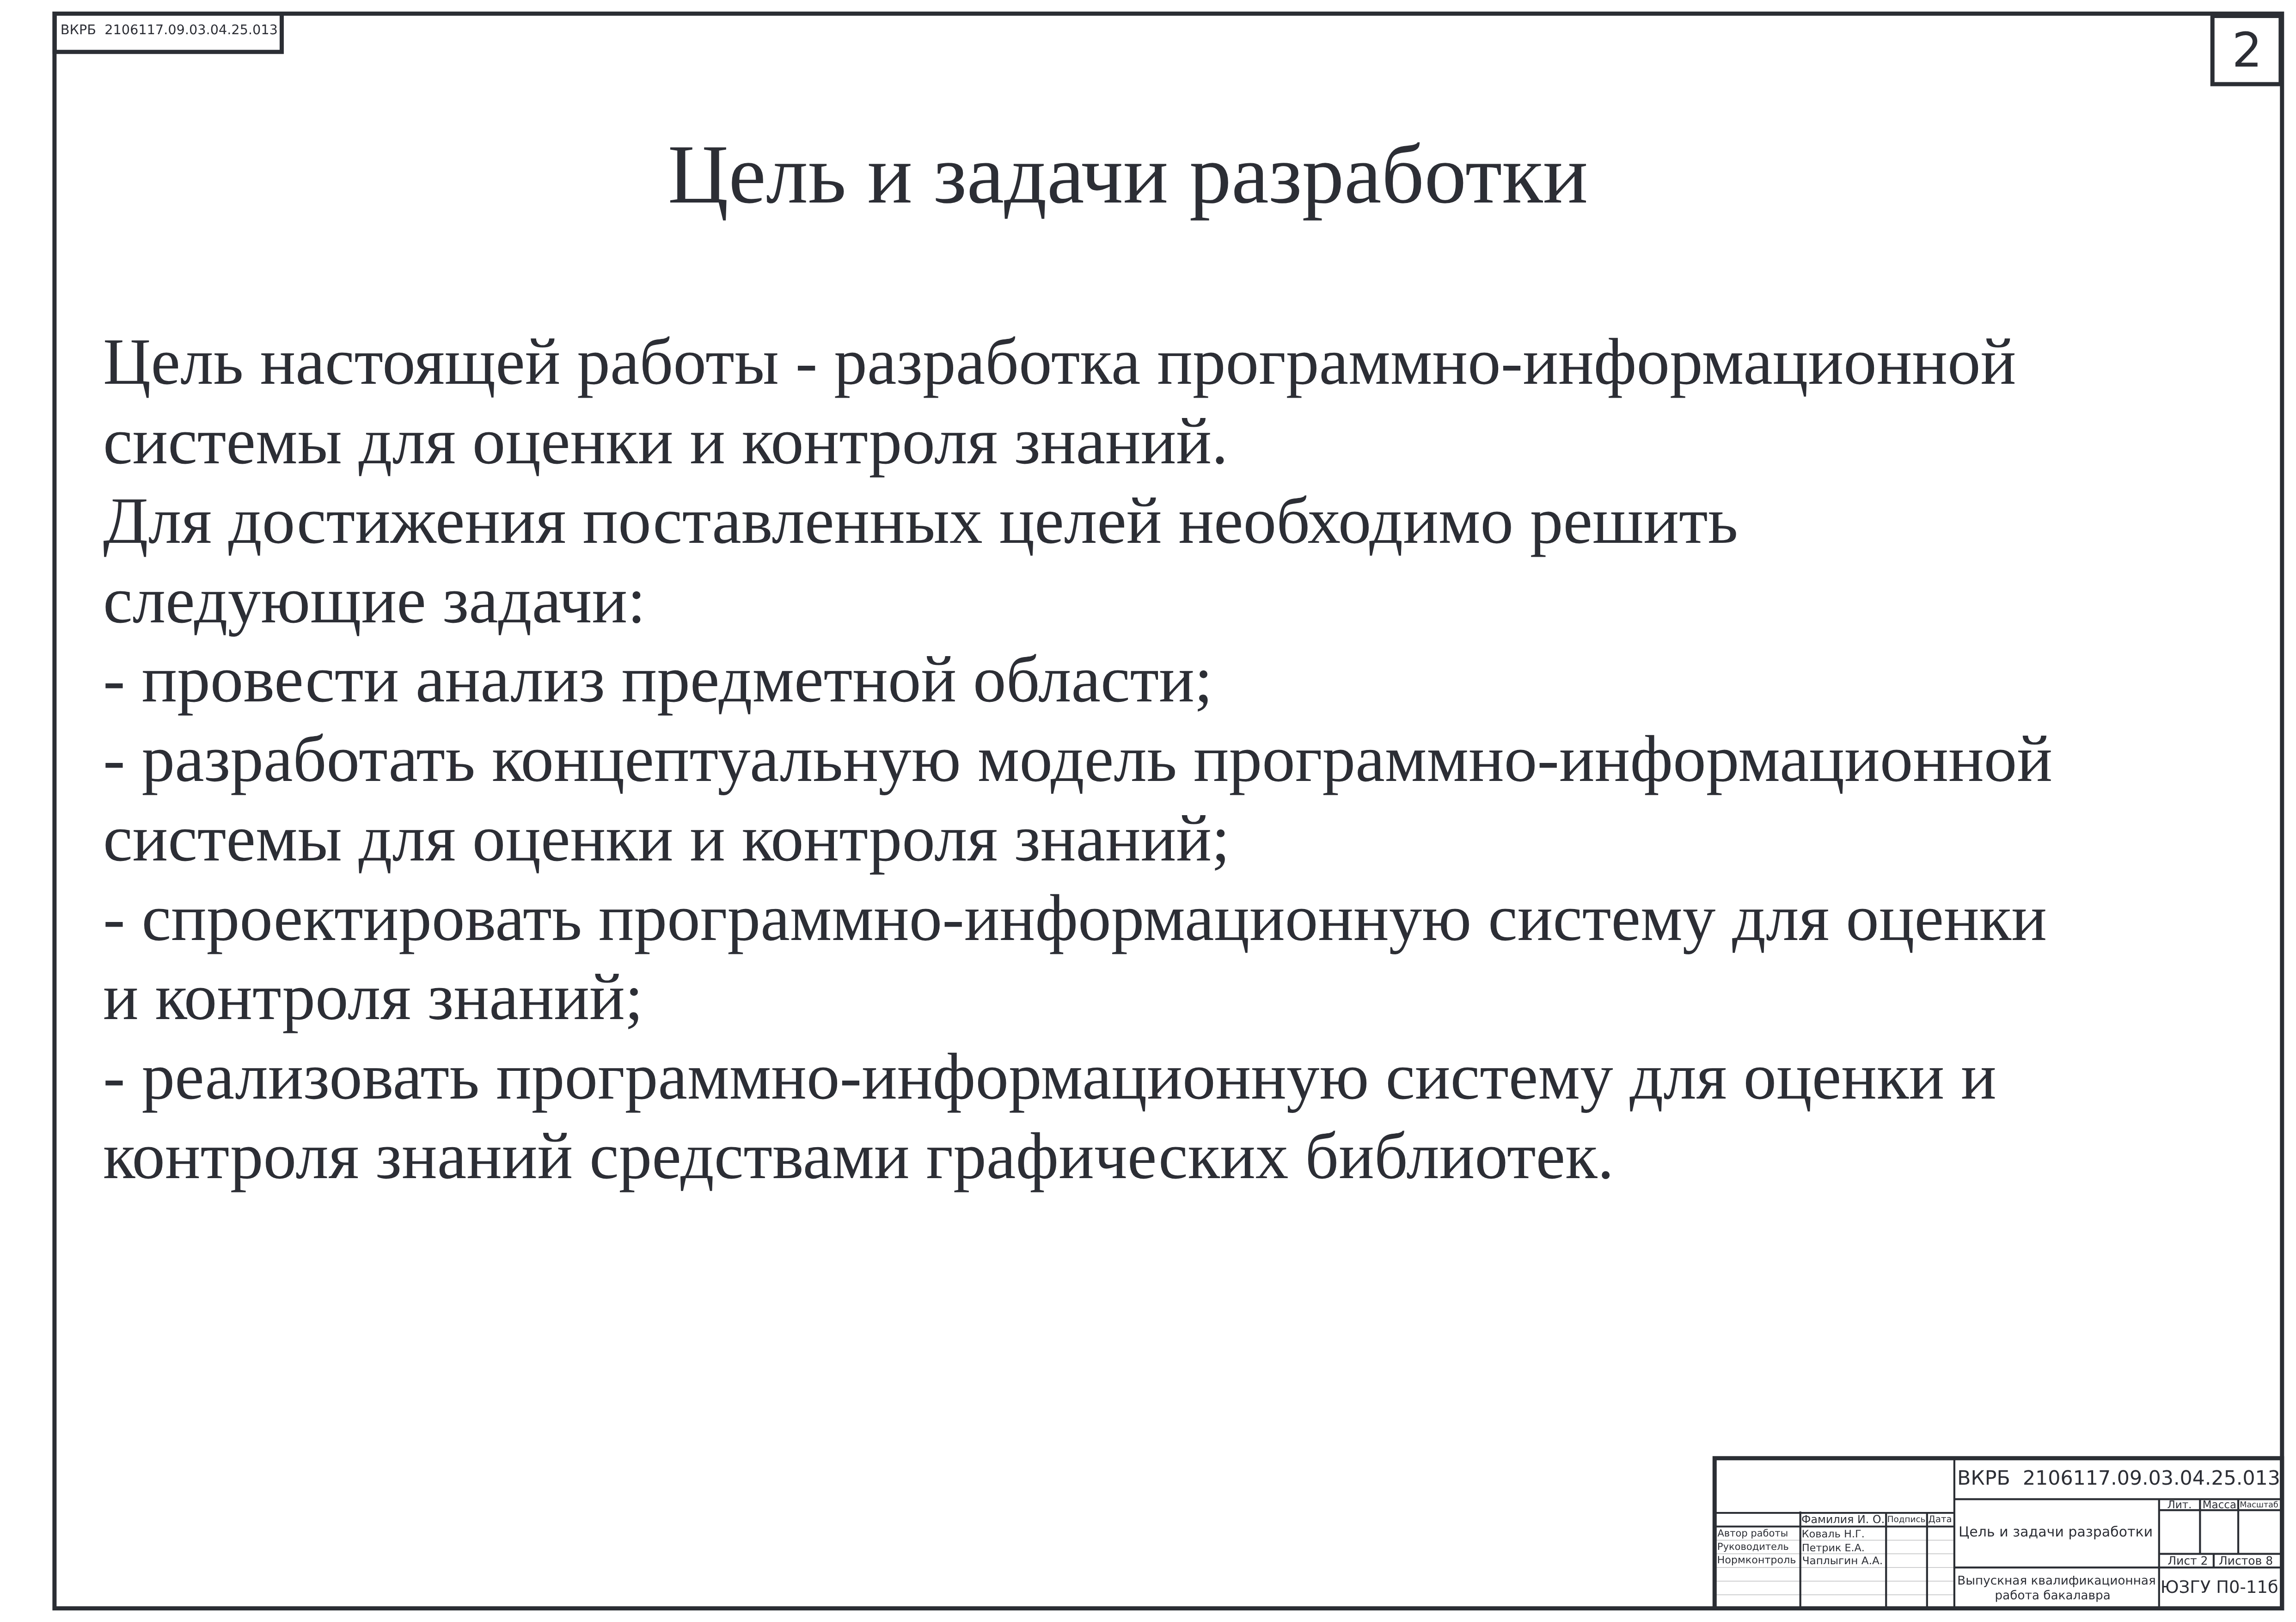
\includegraphics[width=0.82\linewidth]{Плакат_цель_и_задачи.eps}
    \заголовок{Цель и задачи разработки}
    \label{pl2:image}      
\end{плакат}

\begin{плакат}
    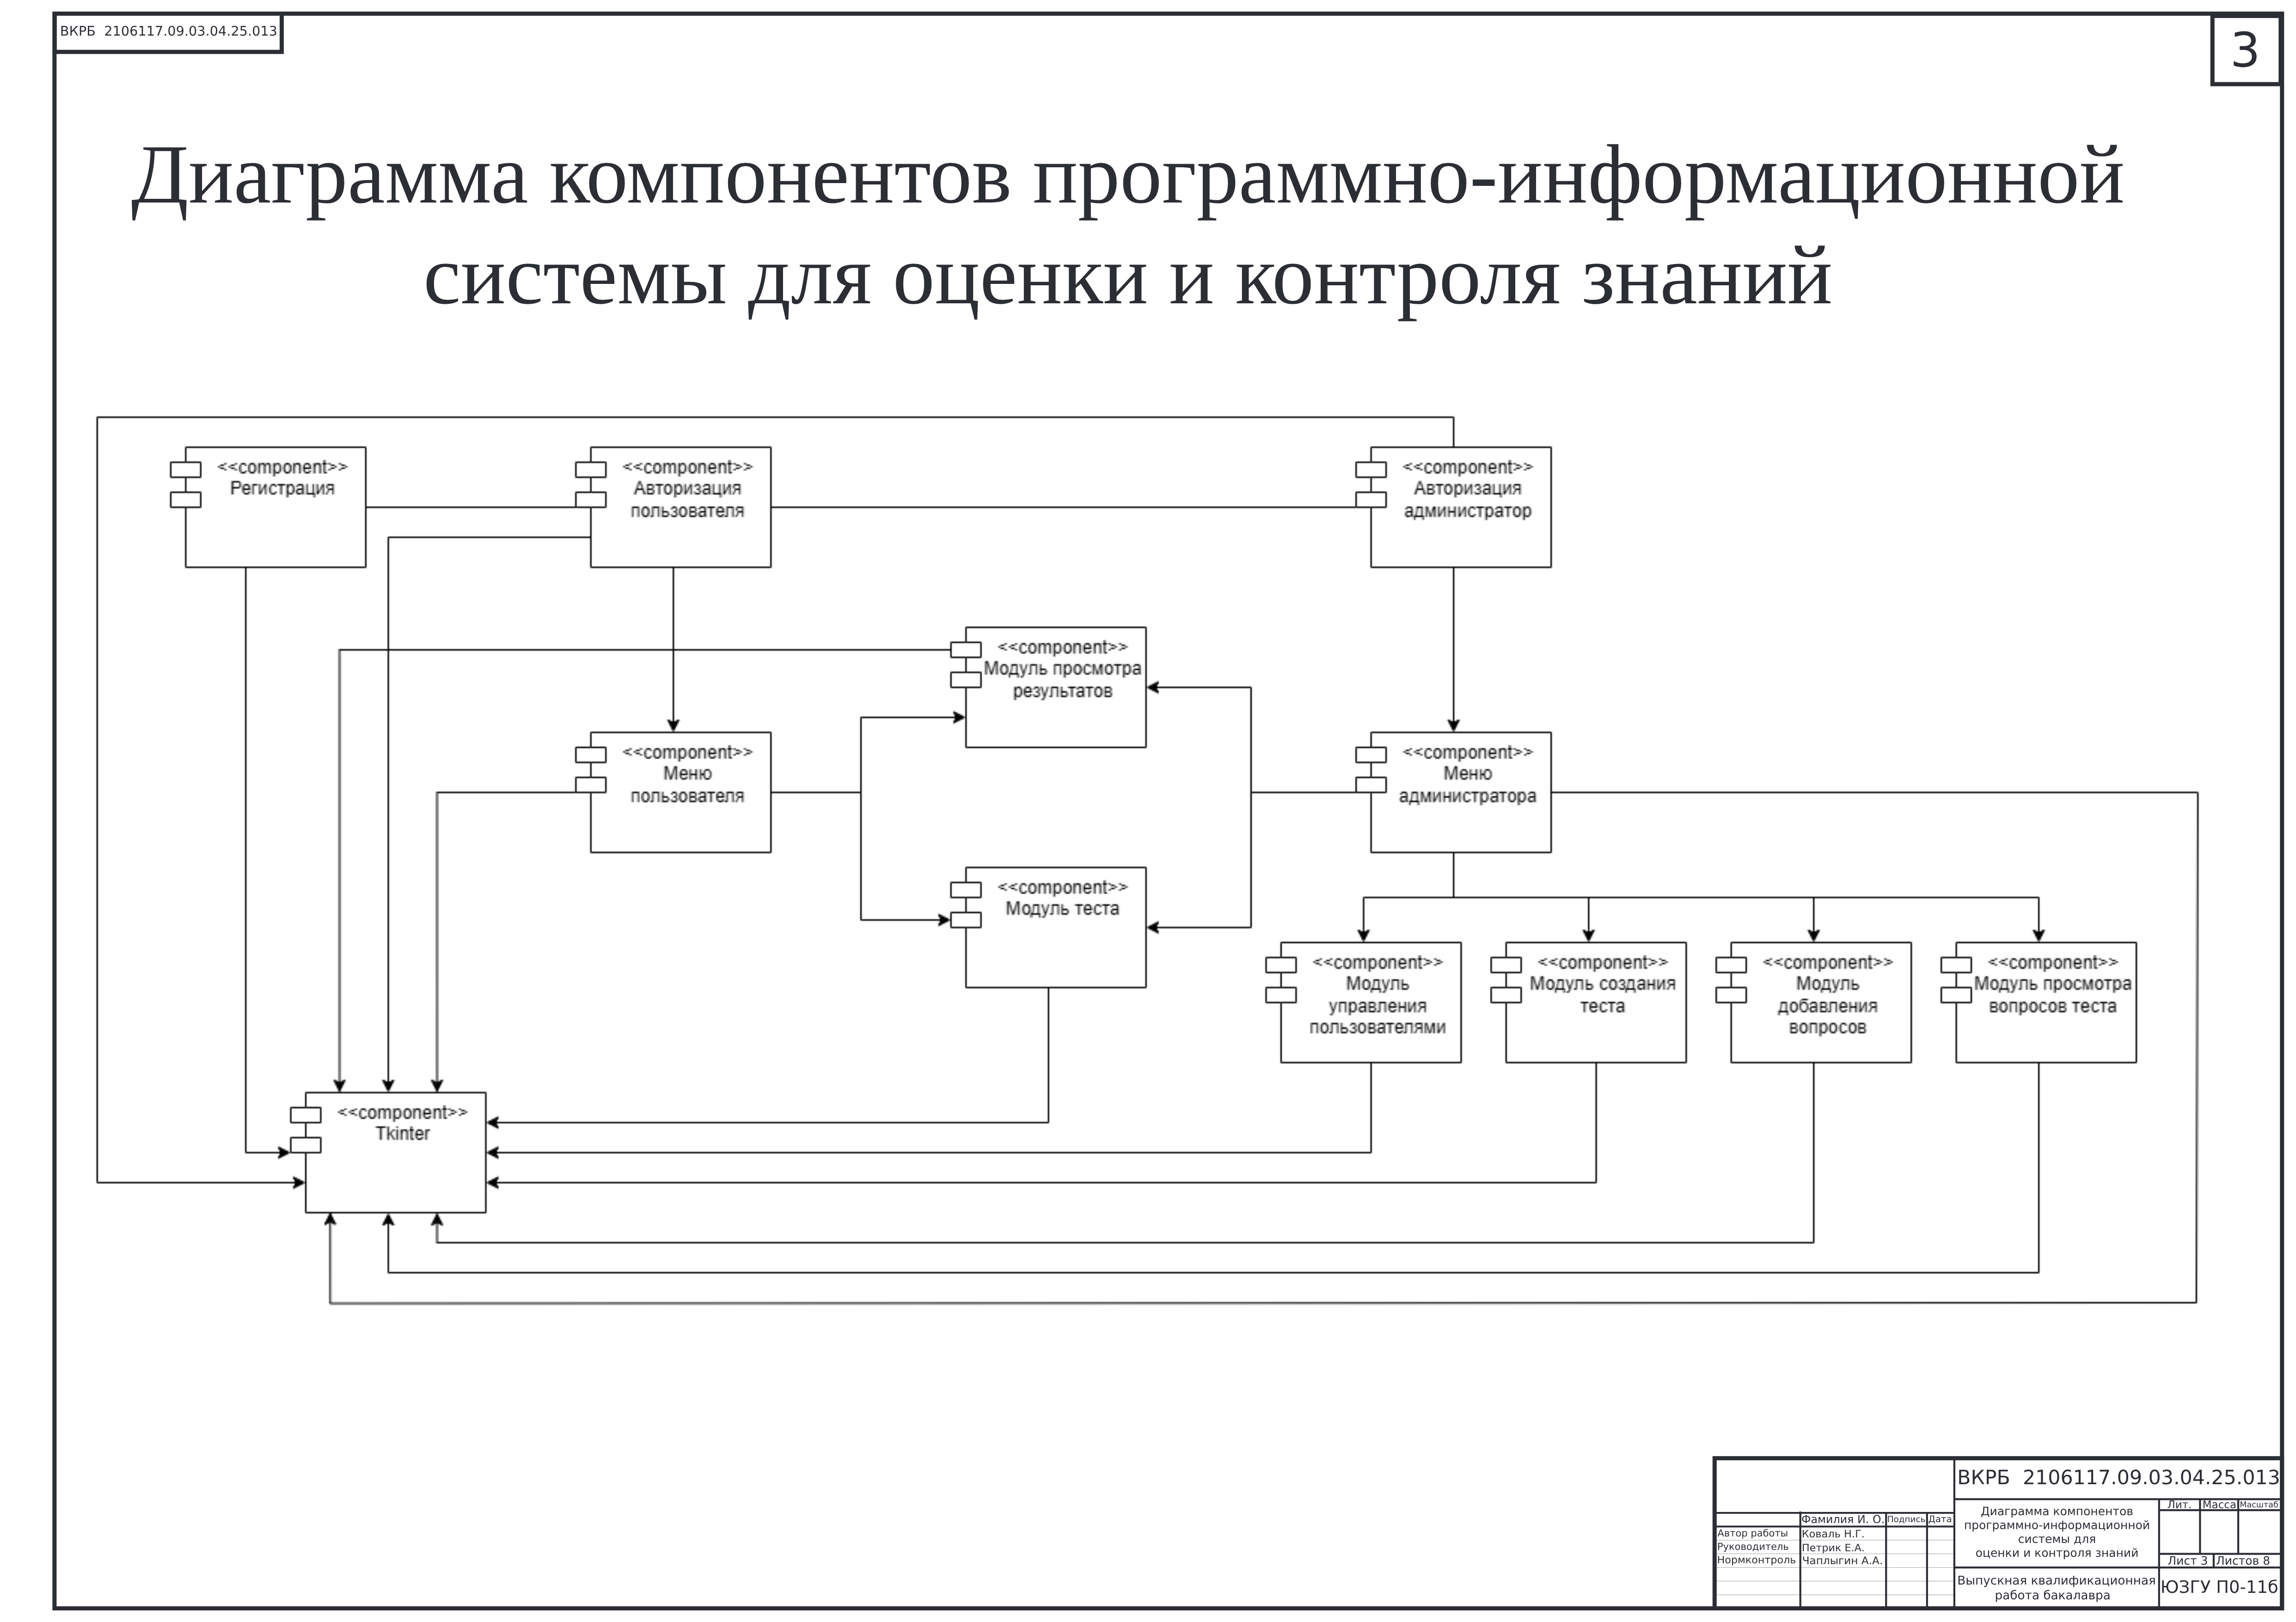
\includegraphics[width=0.82\linewidth]{Плакат_диаграмма_компонентов.eps}
    \заголовок{Диаграмма компонентов}
    \label{pl3:image}      
\end{плакат}

\begin{плакат}
    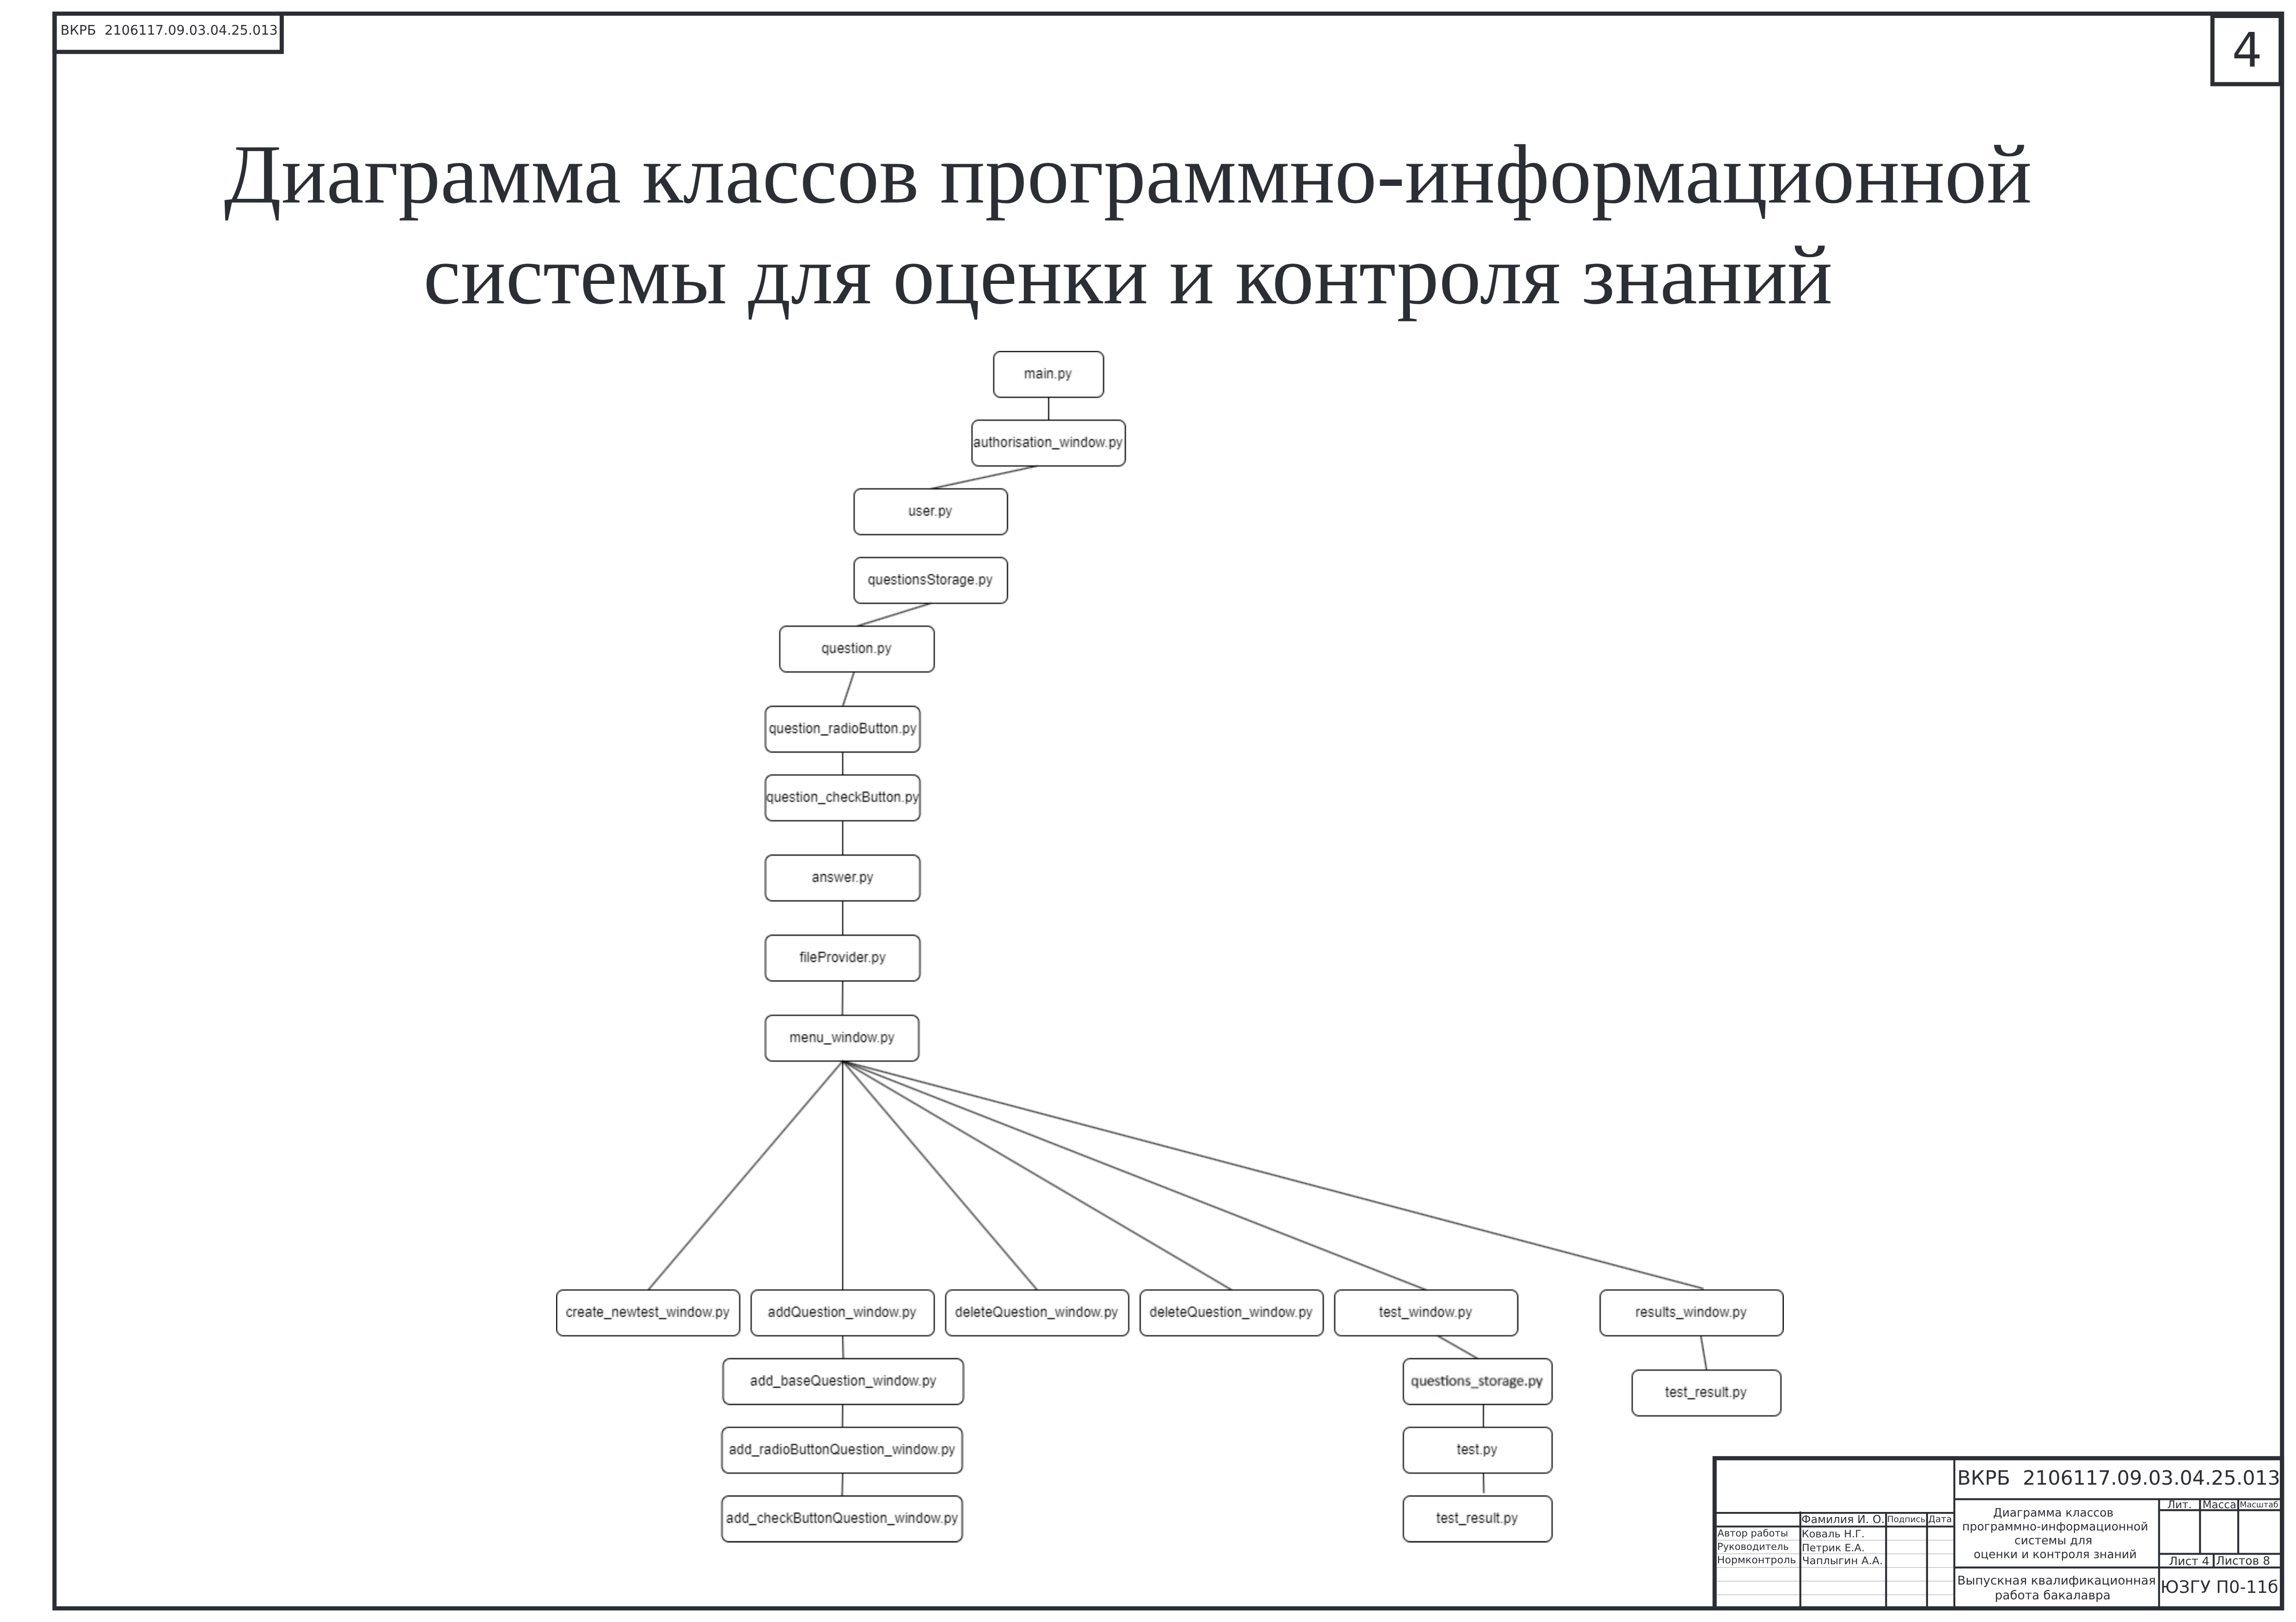
\includegraphics[width=0.82\linewidth]{плакат_диаграмма_классов.eps}
    \заголовок{Диаграмма классов}
    \label{pl4:image}      
\end{плакат}

\begin{плакат}
	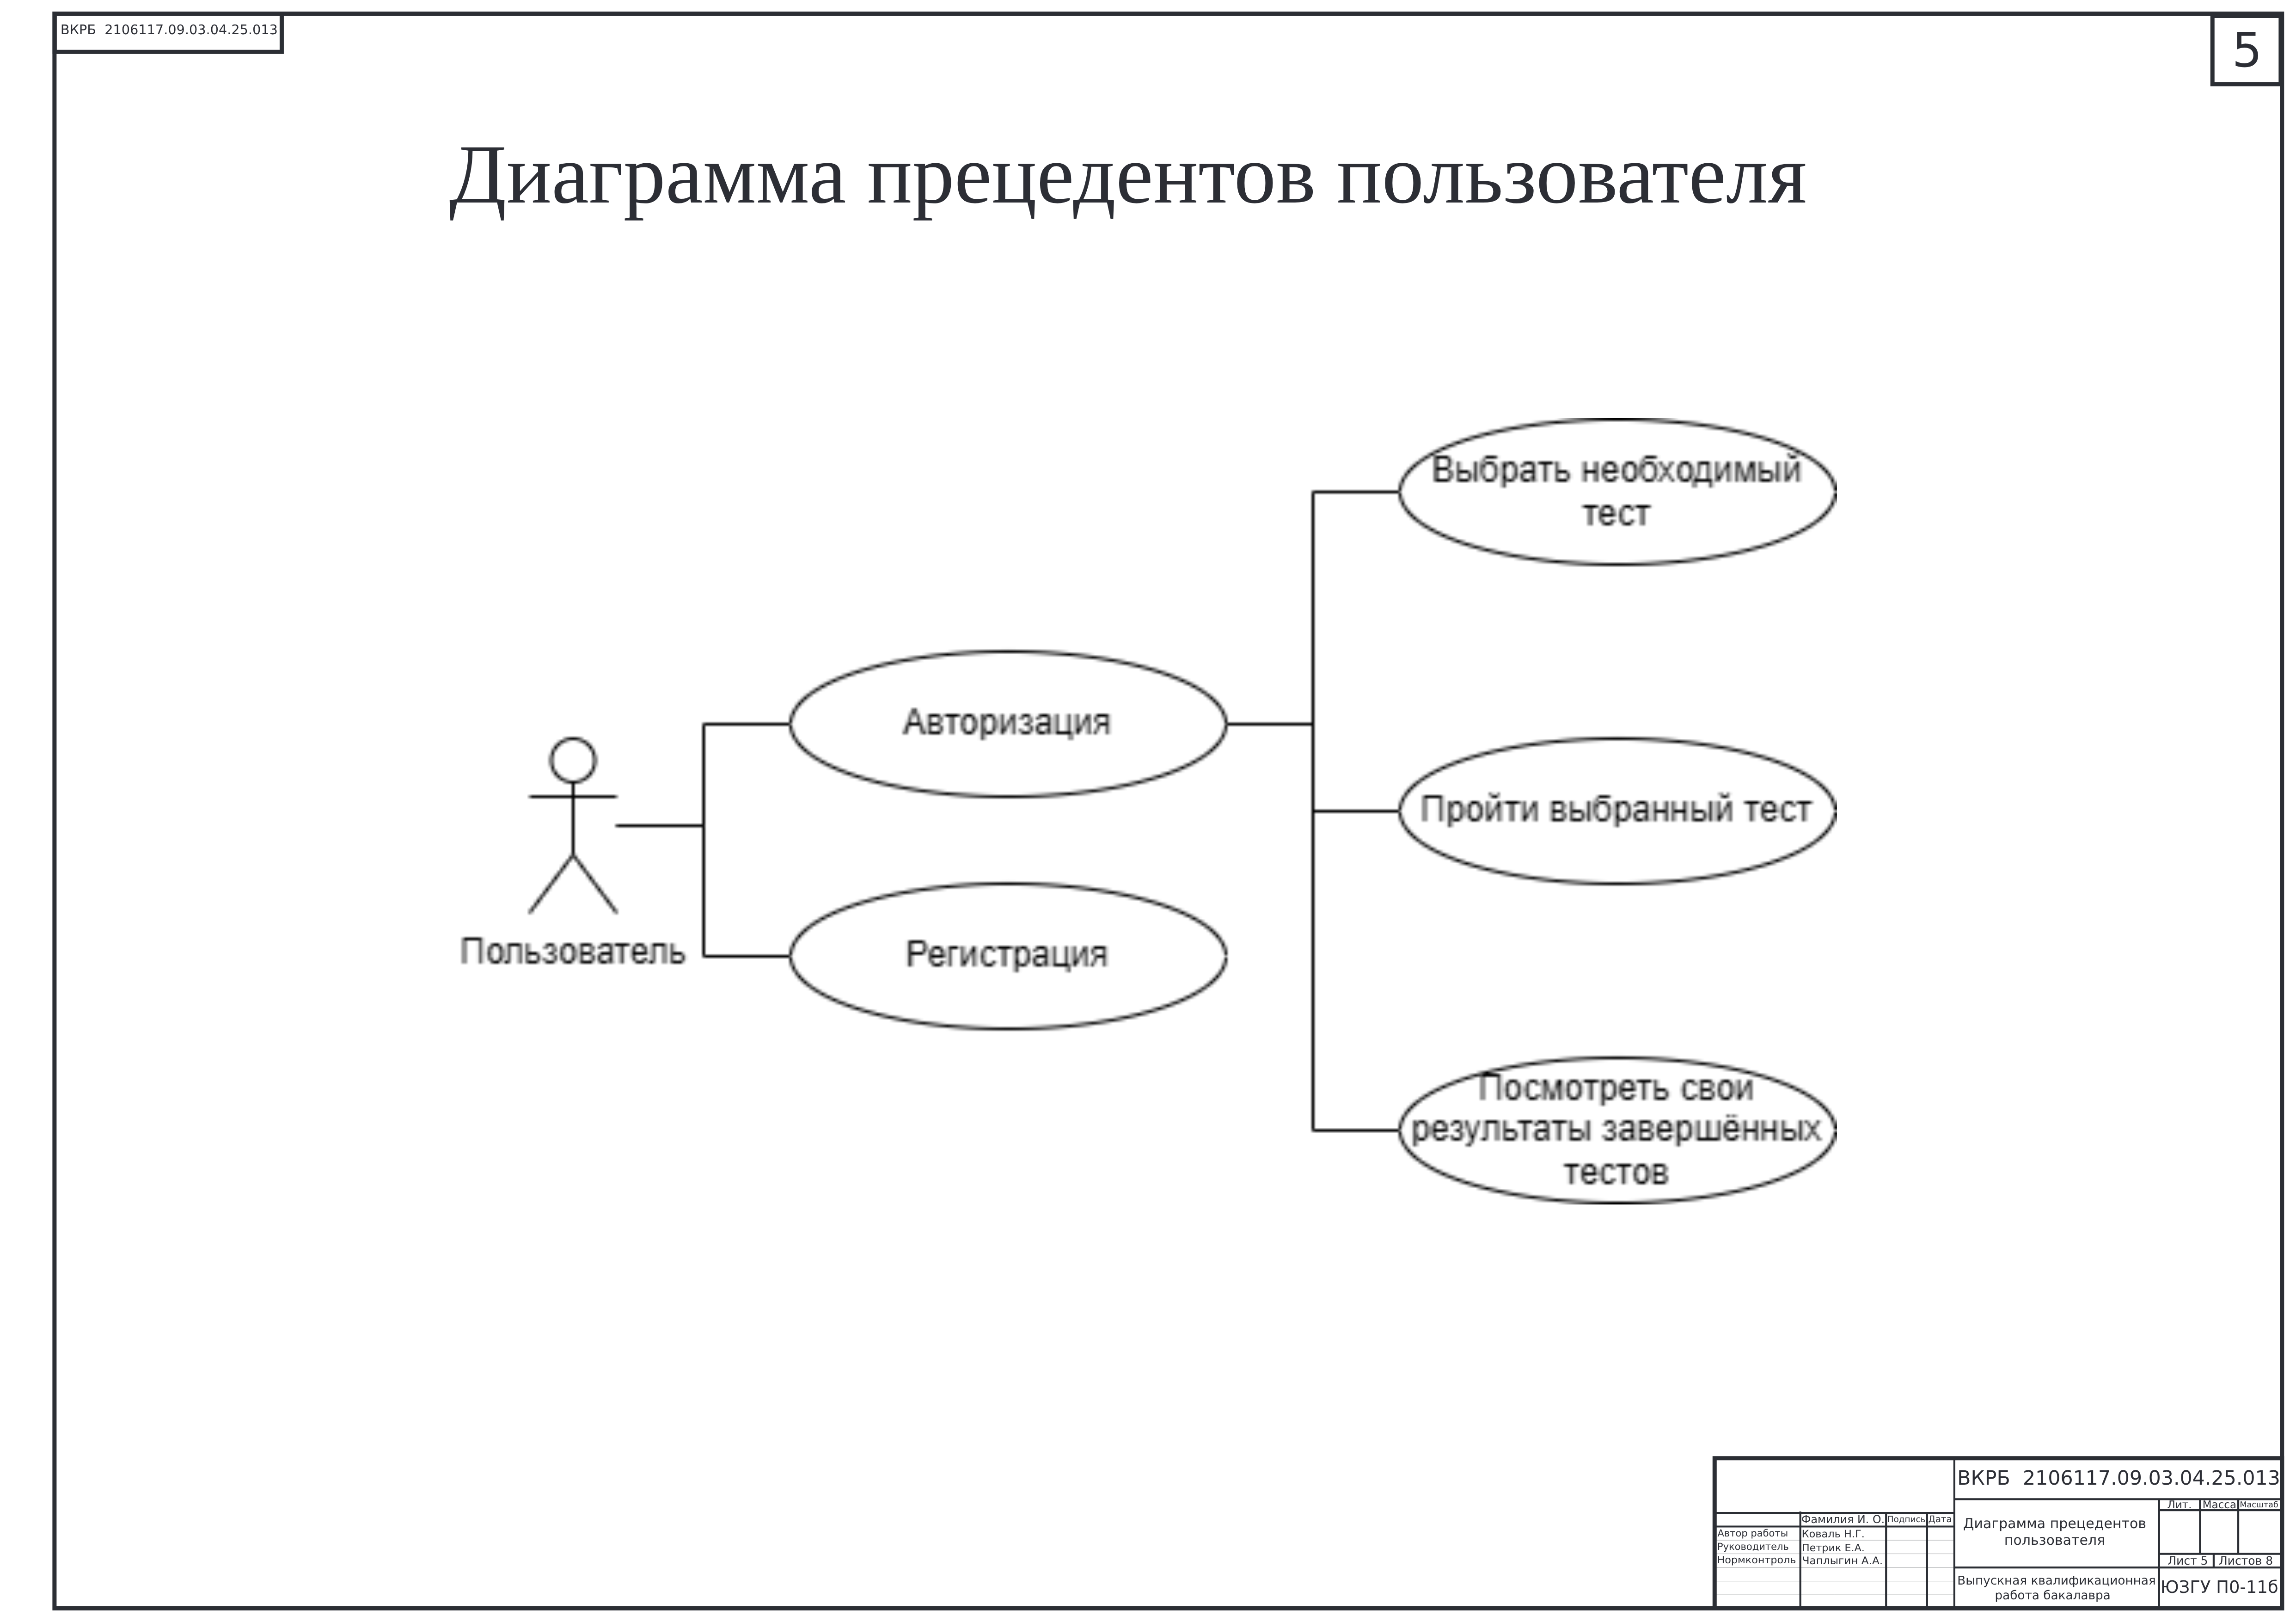
\includegraphics[width=0.82\linewidth]{Плакат_прецеденты_пользователь.eps}
	\заголовок{Прецеденты пользователя}
	\label{pl4:image}      
\end{плакат}

\begin{плакат}
	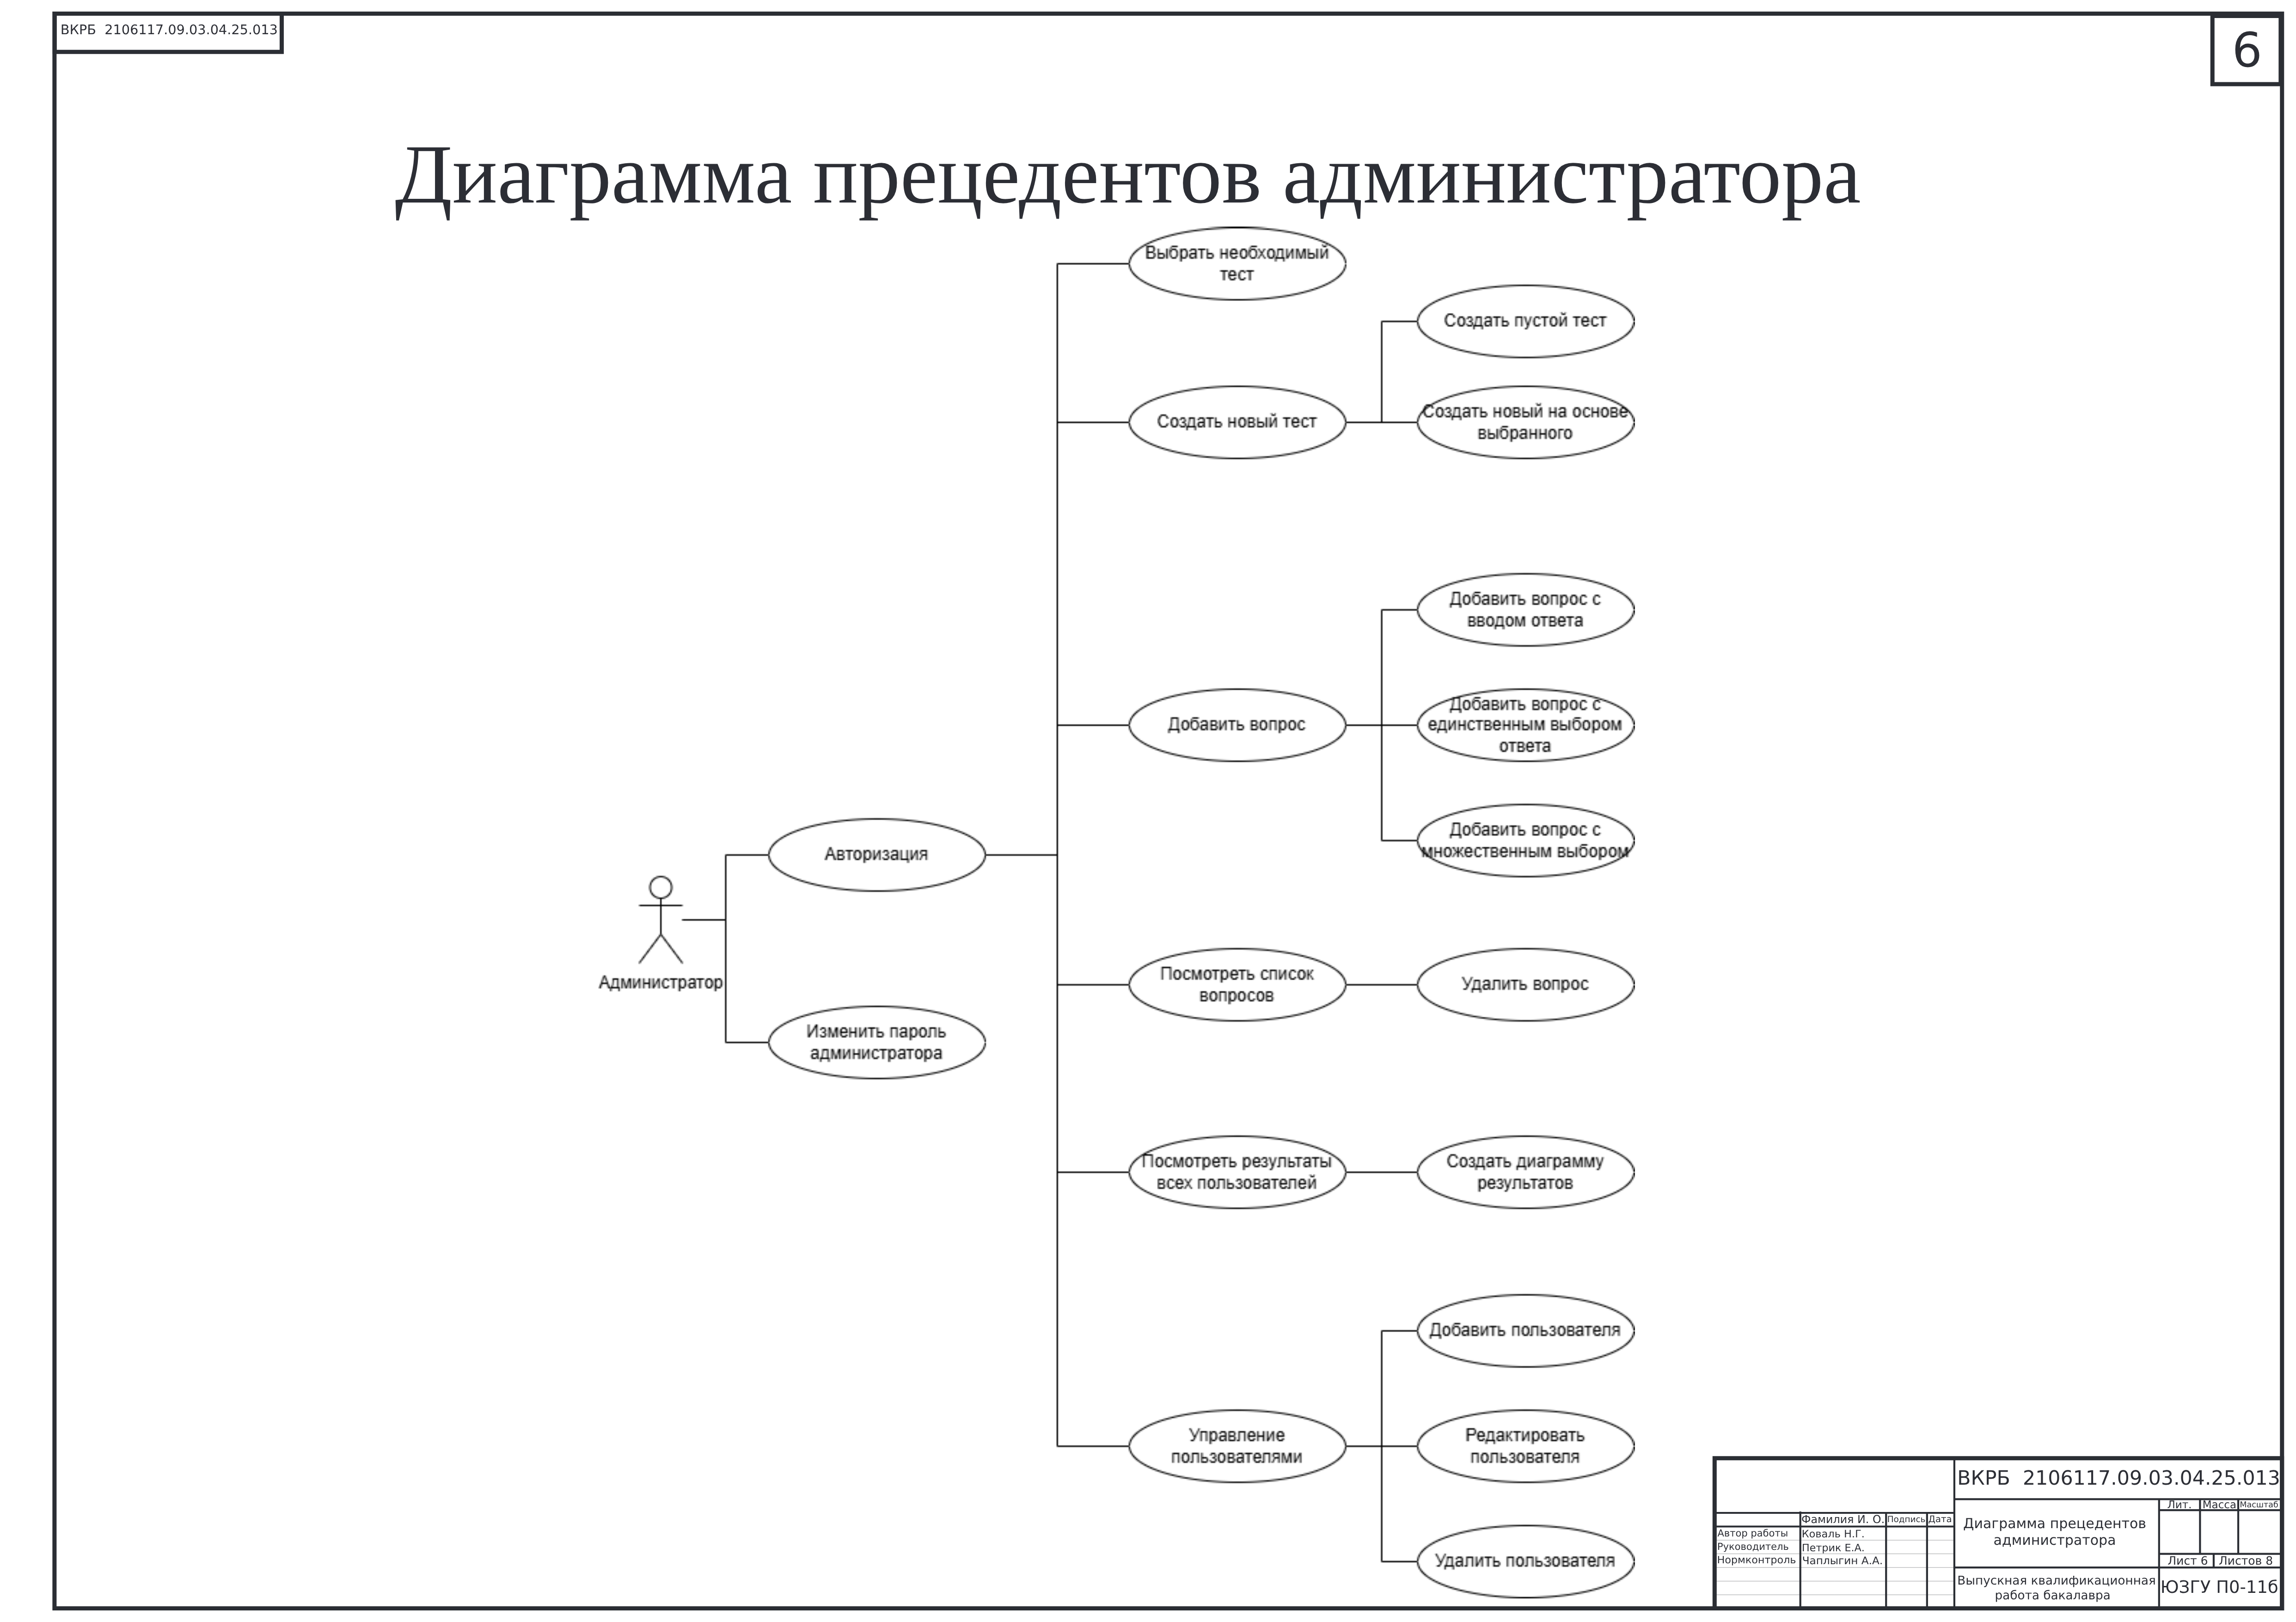
\includegraphics[width=0.82\linewidth]{Плакат_прецеденты_админ.eps}
	\заголовок{Прецеденты администратора}
	\label{pl4:image}      
\end{плакат}

\begin{плакат}
	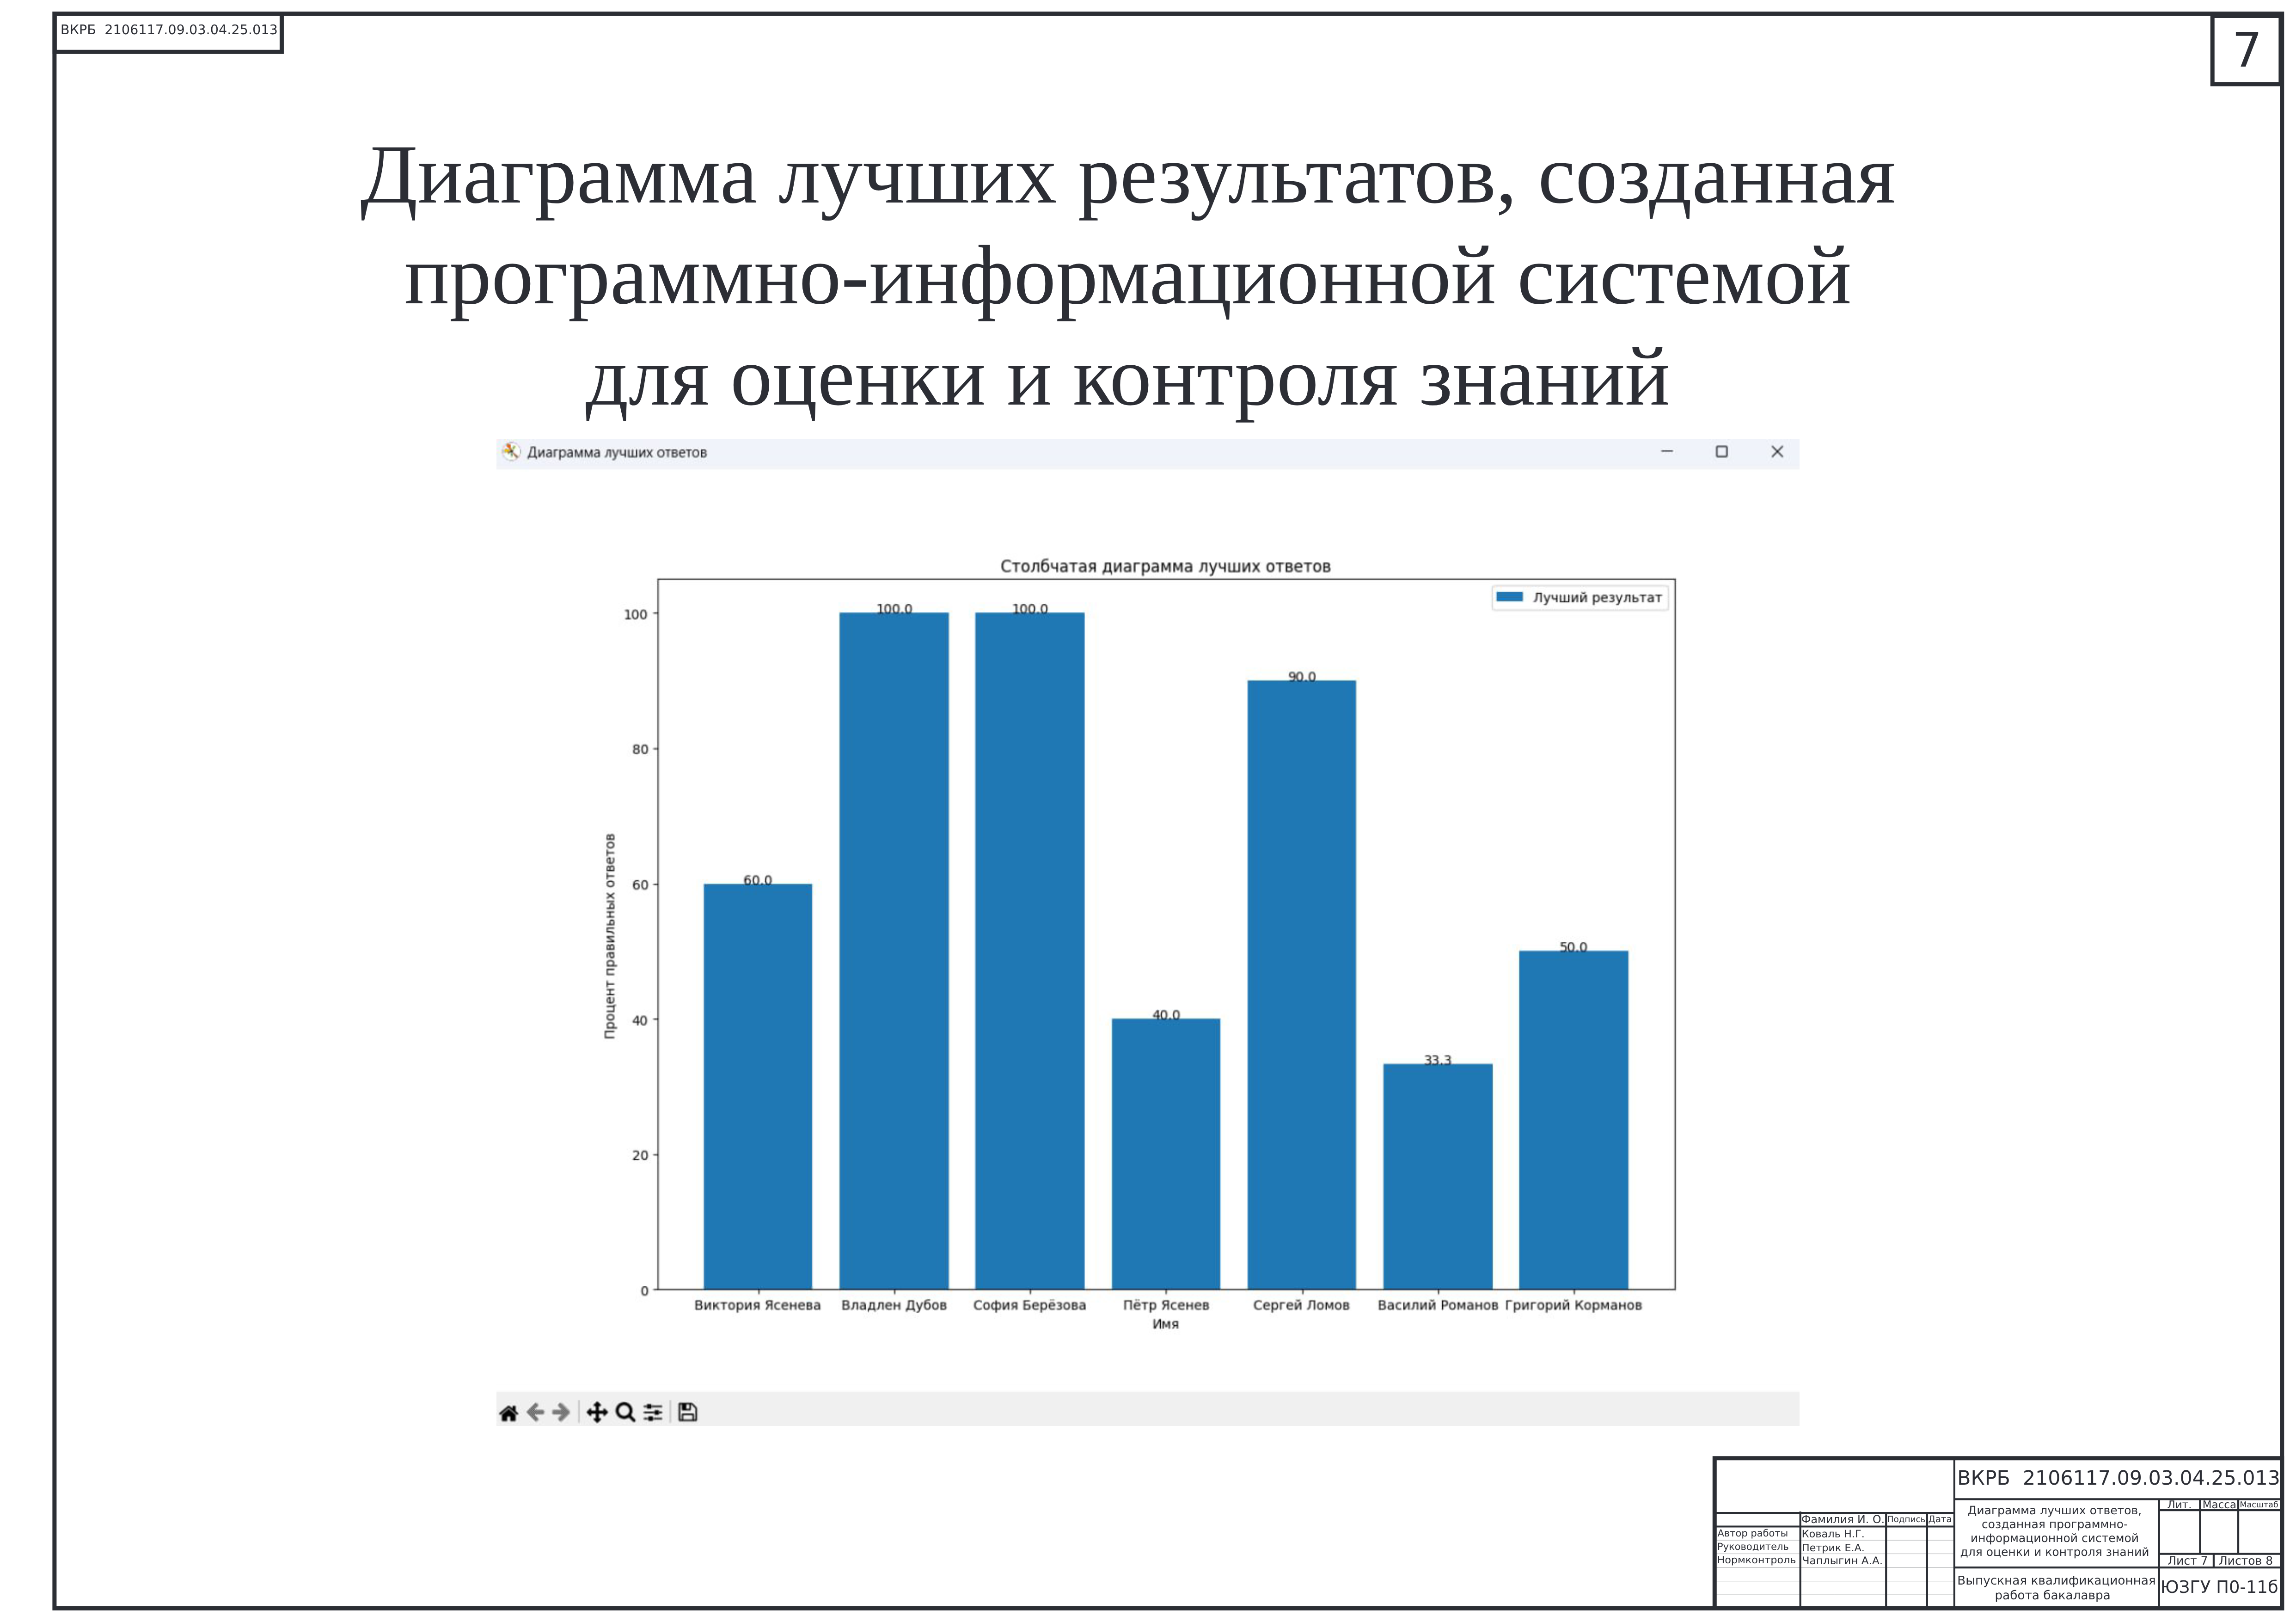
\includegraphics[width=0.82\linewidth]{Плакат_диаграмма_результатов.eps}
	\заголовок{Диаграмма результатов}
	\label{pl4:image}      
\end{плакат}

\begin{плакат}
	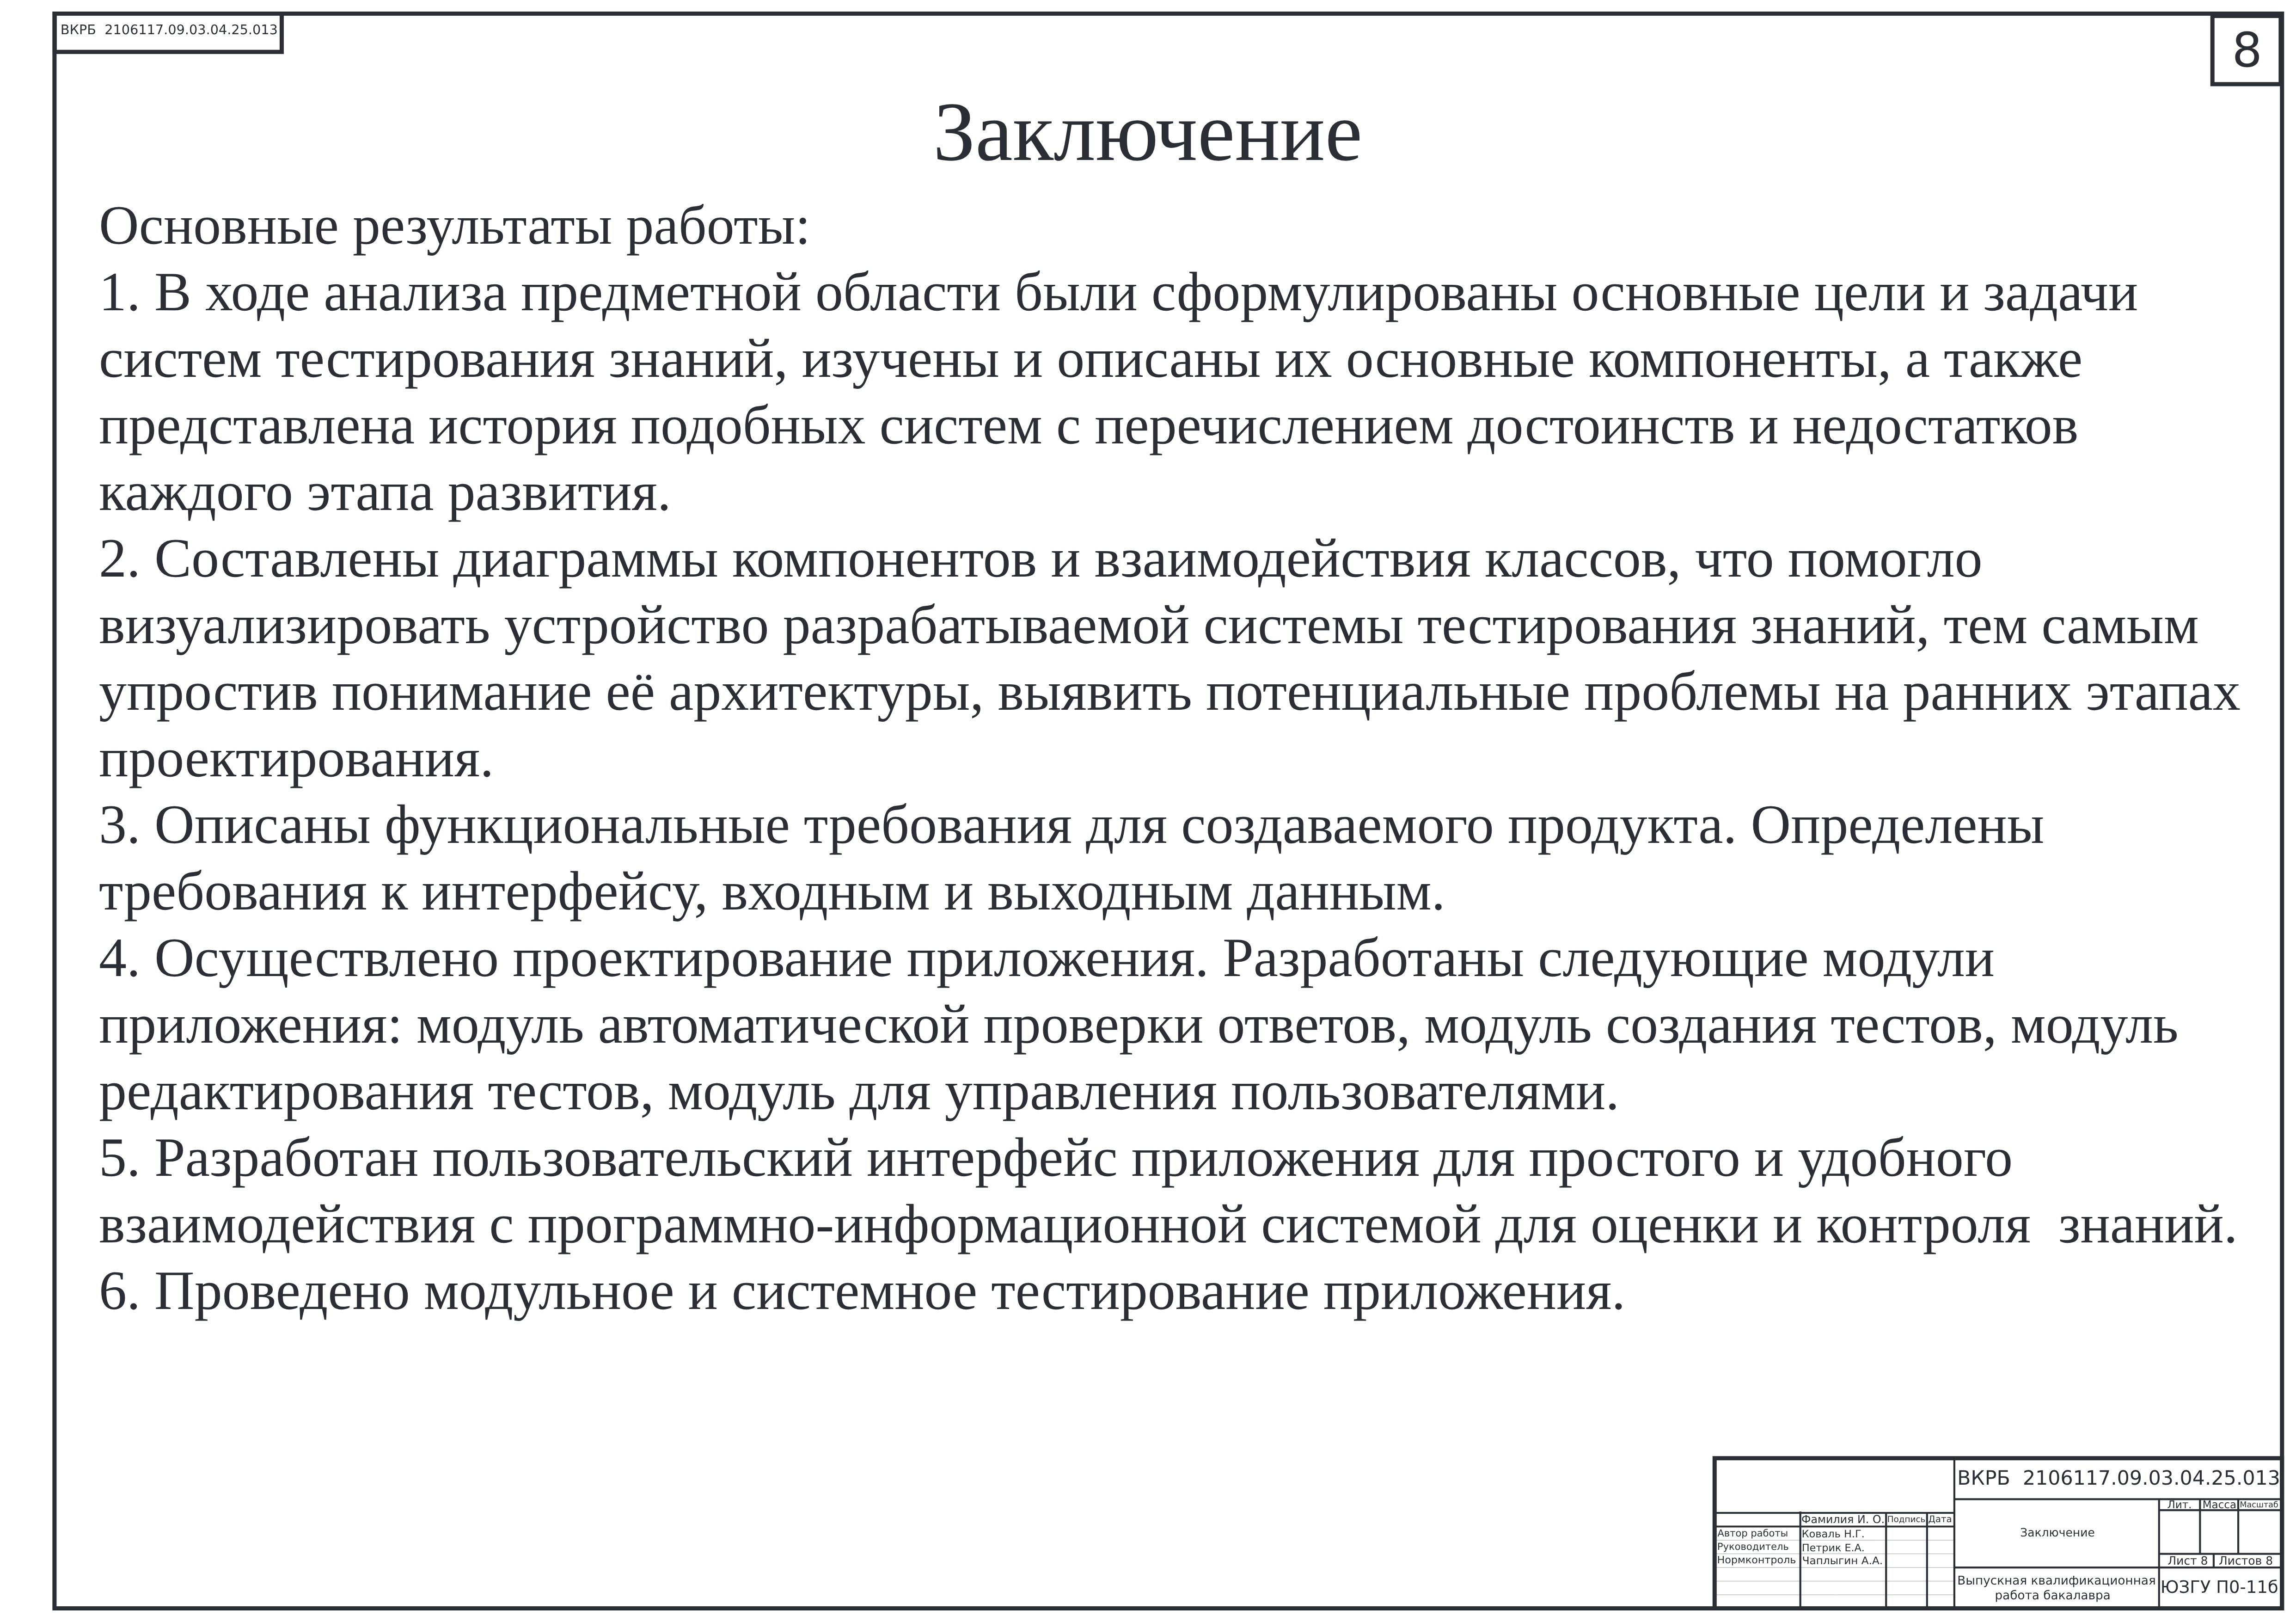
\includegraphics[width=0.82\linewidth]{Плакат_заключение.eps}
	\заголовок{Заключение}
	\label{pl4:image}      
\end{плакат}

\end{landscape}
